\documentclass[a4paper,10pt]{article}
\nonstopmode
\usepackage{amssymb}
\usepackage{longtable}
\usepackage{ifthen}
\usepackage{pgfplots}
\pgfplotsset{compat=1.4}

\textwidth=16.1cm \textheight=27.0cm \topmargin=-1.8cm
\oddsidemargin=0.1cm \evensidemargin=0.1cm \footskip=45pt

\begin{document}

\pgfplotsset{
/pgfplots/log number format basis/.code 2 args={
  \ifdim #1 pt=2pt
    \ifdim #2 pt>0.5pt
      \ifdim #2 pt<10pt
        \pgfmathparse{#1^#2}
        \pgfmathtruncatemacro\r{\pgfmathresult} \r 
      \else
        \ifdim #2 pt<20pt
          \pgfmathparse{#1^(#2 - 10)}
          \pgfmathprintnumber{\pgfmathresult}K
        \else
          \ifdim #2 pt<30pt
            \pgfmathparse{#1^(#2 - 20)}
            \pgfmathprintnumber{\pgfmathresult}M
          \else
            \ifdim #2 pt<40pt
              \pgfmathparse{#1^(#2 - 30)}
              \pgfmathprintnumber{\pgfmathresult}G
            \else
              \ifdim #2 pt<50pt
                \pgfmathparse{#1^(#2 - 40)}
                \pgfmathprintnumber{\pgfmathresult}T
              \else
                \ifdim #2 pt<60pt
                  \pgfmathparse{#1^(#2 - 50)}
                  \pgfmathprintnumber{\pgfmathresult}P
                \else
                  \ifdim #2 pt<70pt
                    \pgfmathparse{#1^(#2 - 60)}
                    \pgfmathprintnumber{\pgfmathresult}E
                  \else
                    >1Z
                  \fi
                \fi
              \fi
            \fi
          \fi
        \fi
      \fi
    \fi
  \fi
  \ifdim #1 pt=10pt
    $#1^{\pgfmathprintnumber{#2}}$
  \fi
}}

\begin{titlepage}\thispagestyle{empty}
\begin{huge}\begin{flushleft}\bf{OTF Profile}\end{flushleft}\end{huge}
\hrule
\begin{flushright}\textbf{\large Trace Properties}\end{flushright}
\vspace{0.5\baselineskip}
\begin{flushleft}
\begin{tabular}{ll}
\bf{OTF Version:} & \verb|1.11.1openmpi| \\
\bf{Creator:} & \verb|VampirTrace 5.13.1openmpi|\\
\bf{File:} & \verb|RoadMapProf_static.otf|
\end{tabular}

\vspace{1\baselineskip}
\begin{tabular}{ll}
\bf{Number of Processes:} & \verb|6|\\
\bf{Timer Resolution:} & \verb|3.59135 GHz|
\end{tabular}

\vspace{1\baselineskip}
\begin{tabular}{l}\bf{Comments:}\end{tabular}
\begin{quote}\begin{verbatim}
Trace Times:
 Start: Wed Sep 16 00:31:39 2015 (1442356299868475)
 Stop: Wed Sep 16 00:31:48 2015 (1442356308409705)
 Elapsed: 00:00:08 (8541230)
VampirTrace Environment:
 VT_MODE: TRACE
 VT_BUFFER_SIZE: 32M
 VT_SYNC_FLUSH: no
 VT_SYNC_FLUSH_LEVEL: 80
 VT_SNAPSHOTS: yes
 VT_MAX_SNAPSHOTS: 1024
 VT_ONOFF_CHECK_STACK_BALANCE: yes
 VT_MAX_STACK_DEPTH: 0
 VT_MAX_FLUSHES: 50
 VT_RUSAGE: <not set>
 VT_MPITRACE: yes
 VT_MEMTRACE: no
 VT_CPUIDTRACE: no
 VT_IOTRACE: no
 VT_IOTRACE_EXTENDED: no
 VT_PTHREAD_REUSE: yes
 VT_FILTER_SPEC: mpivt_filter
 VT_GROUPS_SPEC: <not set>
\end{verbatim}\end{quote}
\end{flushleft}
\vspace*{\fill}
\begin{flushright}\today\end{flushright}
\end{titlepage}

\newpage

\begin{center}\small
{\Large \bf Top 12 of 12 Functions}
\bigskip
\begin{longtable}{|l||r|r|r|}

   \hline
   \bf Function & \bf invocations[\#] & \bf excl. time[sec] $\nabla$ & \bf incl. time[sec] \\
   \hline\hline
  \verb|RoadMap| &   \verb|6| &   \verb|23.1318| &   \verb|45.5133| \\
  \verb|MPI_Barrier| &   \verb|60| &   \verb|12.4361| &   \verb|12.4361| \\
  \verb|MPI_Recv| &   \verb|8 000| &   \verb|7.20719| &   \verb|7.20719| \\
      \hline
  \verb|MPI_Init| &   \verb|6| &   \verb|2.56581| &   \verb|2.63467| \\
  \verb|CreateMap| &   \verb|510| &   \verb|1.67327| &   \verb|10.5095| \\
  \verb|MPI_Send| &   \verb|8 000| &   \verb|1.06495| &   \verb|1.06495| \\
      \hline
  \verb|main| &   \verb|6| &   \verb|0.58333| &   \verb|48.7933| \\
  \verb|sync time| &   \verb|12| &   \verb|0.129503| &   \verb|0.129503| \\
  \verb|MPI_Finalize| &   \verb|6| &   \verb|0.00105601| &   \verb|0.0616988| \\
      \hline
  \verb|setup_colors| &   \verb|6| &   \verb|0.000200889| &   \verb|0.000200889| \\
  \verb|MPI_Comm_rank| &   \verb|66| &   \verb|2.94117e-05| &   \verb|2.94117e-05| \\
  \verb|MPI_Comm_size| &   \verb|60| &   \verb|1.42036e-05| &   \verb|1.42036e-05| \\
   \hline
\end{longtable}

\end{center}
\newpage

\begin{center}
{\Large \bf Top 50 Dispersion of Functions (in seconds)}
\bigskip
\end{center}
\newcounter{shiftctr}
\newlength{\lowqpos}
\newlength{\medianpos}
%#1: min, #2: 1/4 quartile, #3: 1/4pos, #4: median, #5: medianpos, #6: 3/4 quartile, #7: 3/4pos, #8: max
\newcommand{\boxplotlh}[8]{
\begin{tikzpicture}
\begin{small}
  % set all counters and lengths to zero
  \setcounter{shiftctr}{0}
  \setlength{\lowqpos}{#3 pt}
  \addtolength{\lowqpos}{3pt}
  \setlength{\medianpos}{#5 pt}
  \addtolength{\medianpos}{3pt}
  \filldraw[fill=green!20] (#3,0) rectangle (#7,0.5);% box
  \draw (0,0) node[below]{$t_{min}:#1$} -- (0,0.5);
  \draw (0,0.25) -- (#3,0.25);% left whisker

  % check overlap of lower quartile label
  \ifdim #3 pt > 10pt
    \addtocounter{shiftctr}{4}
  \else
    \ifdim #3 pt < 2pt
      \addtocounter{shiftctr}{4}
    \fi
  \fi
  \node at (#3,0) [below,yshift=-\theshiftctr mm] {$t_{1/4}:#2$};

  % check overlap of median label
  \ifdim #5 pt > 10pt
    \addtocounter{shiftctr}{4}
  \else
    \ifnum\theshiftctr=4
      \ifdim #5 pt < 3pt
        \addtocounter{shiftctr}{4}
      \else
        \setcounter{shiftctr}{0}
      \fi
    \else
      \ifdim #5 pt < \lowqpos
        \addtocounter{shiftctr}{4}
      \fi
    \fi
  \fi
  \draw[color=red] (#5,0.5) -- (#5,0) node[below,color=black,yshift=-\theshiftctr mm]{$t_{med}:#4$};

% check overlap of higher quartile label
  \ifdim #7 pt > 10pt
    \addtocounter{shiftctr}{4}
  \else
    \ifnum\theshiftctr>0
      \ifdim #7 pt < \lowqpos
        \addtocounter{shiftctr}{4}
      \else
        \setcounter{shiftctr}{0}
      \fi
    \else
      \ifdim #7 pt < \medianpos
        \addtocounter{shiftctr}{4}
      \fi
    \fi
  \fi
  \node at (#7,0) [below,yshift=-\theshiftctr mm] {$t_{3/4}:#6$};

  \draw (#7,0.25) -- (13,0.25);% right whisker
  \draw (13,0.5) -- (13,0) node[below]{$t_{max}:#8$};
\end{small}
\end{tikzpicture}
}
\begin{flushleft}
\end{flushleft}

\newpage

\newpage

\begin{flushright}\ttfamily\small
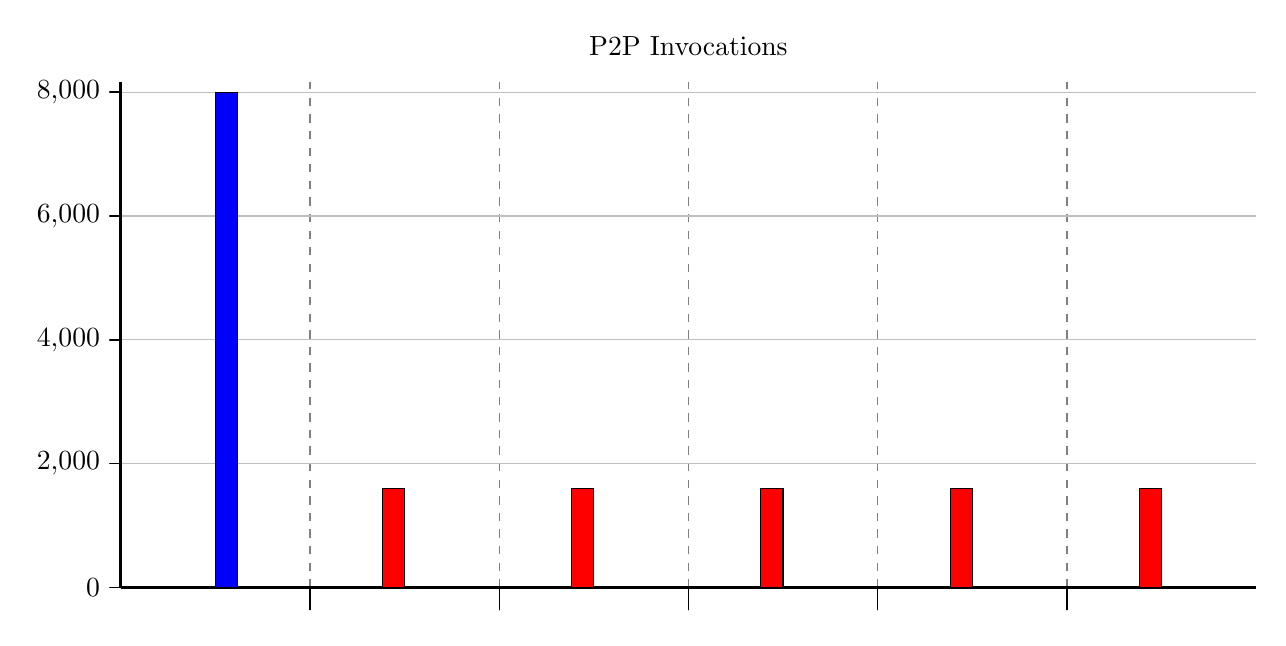
\begin{tikzpicture}
\begin{axis}[
  width=16cm, height=8cm,
  axis x line=bottom,x axis line style={-,line width=1pt},
  axis y line=left,y axis line style={-,line width=1pt},
  enlarge y limits={value=0.02,upper},
  ymin=0,ymajorgrids,xminorgrids,minor x tick num=1,
title=P2P Invocations,ylabel={},
x tick label style={rotate=90,anchor=east,font=\ttfamily\footnotesize},
tick align=outside,
tick style={line cap=round,line width=0.5pt,color=black,
      major tick length=4pt,minor tick length=8pt},
major x tick style={line width=1, color=white},
scaled y ticks=true,
bar width=8pt,
minor grid style={color=gray, line width=0.5pt, dashed},
xmin=-0.5,
xmax=5.5,
xtick={0,...,5},
xticklabels={
},]
\addplot[ybar, draw=black, mark=none, fill=red, xshift=-4]
  coordinates{
(1,1600)(2,1600)(3,1600)(4,1600)(5,1600)};
\addplot[ybar, draw=black, mark=none, fill=blue, xshift=4]
  coordinates{
(0,8000)};
\end{axis}
\end{tikzpicture}

\end{flushright}
\begin{flushright}\ttfamily\small
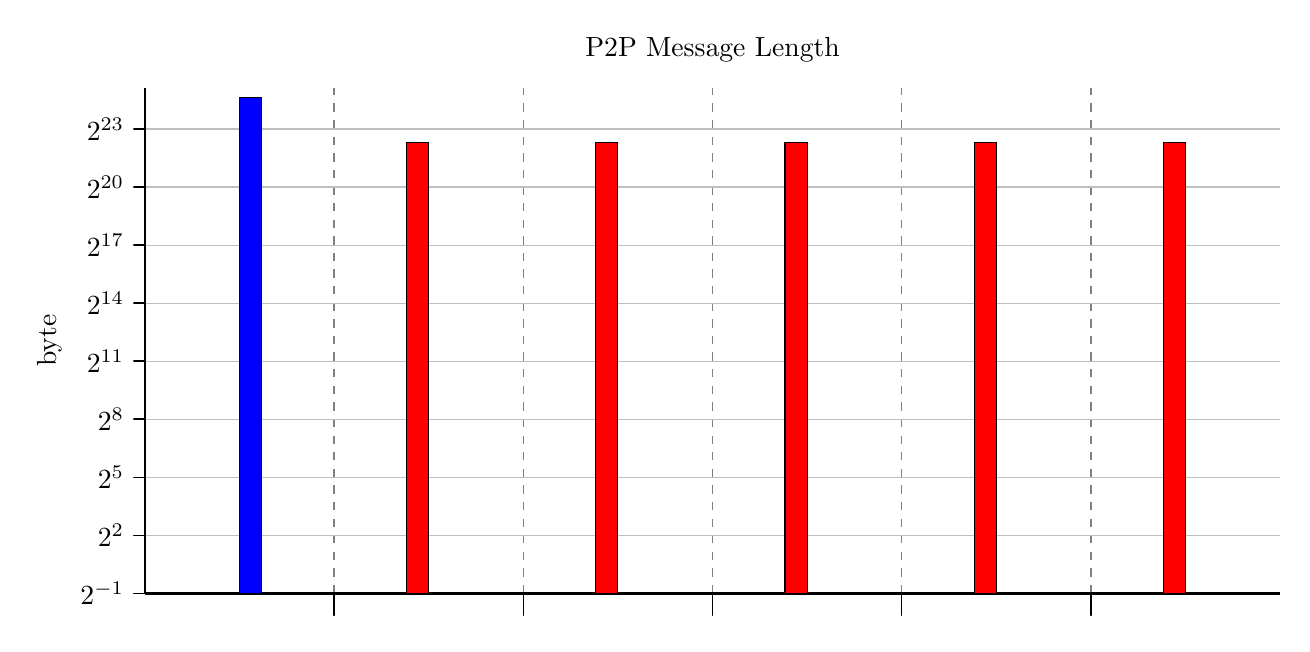
\begin{tikzpicture}
\def \ymin {0.5}
\begin{axis}[
  width=16cm, height=8cm,
  axis x line=bottom,x axis line style={-,line width=1pt},
  axis y line=left,y axis line style={-,line width=1pt},
  enlarge y limits={value=0.02,upper},
  ymode=log,log basis y=2,ymin=\ymin,
  try min ticks log={8},
ymajorgrids,xminorgrids,minor x tick num=1,
title=P2P Message Length,ylabel={byte},
x tick label style={rotate=90,anchor=east,font=\ttfamily\footnotesize},
tick align=outside,
tick style={line cap=round,line width=0.5pt,color=black,
      major tick length=4pt,minor tick length=8pt},
major x tick style={line width=1, color=white},
scaled y ticks=true,
bar width=8pt,
minor grid style={color=gray, line width=0.5pt, dashed},
xmin=-0.5,
xmax=5.5,
xtick={0,...,5},
xticklabels={
},]
\addplot[ybar, draw=black, mark=none, fill=red, xshift=-4]
  coordinates{
(1,5126400)(2,5126400)(3,5126400)(4,5126400)(5,5126400)};
\addplot[ybar, draw=black, mark=none, fill=blue, xshift=4]
  coordinates{
(0,25632000)};
\end{axis}
\end{tikzpicture}

\end{flushright}
\begin{flushright}\ttfamily\small
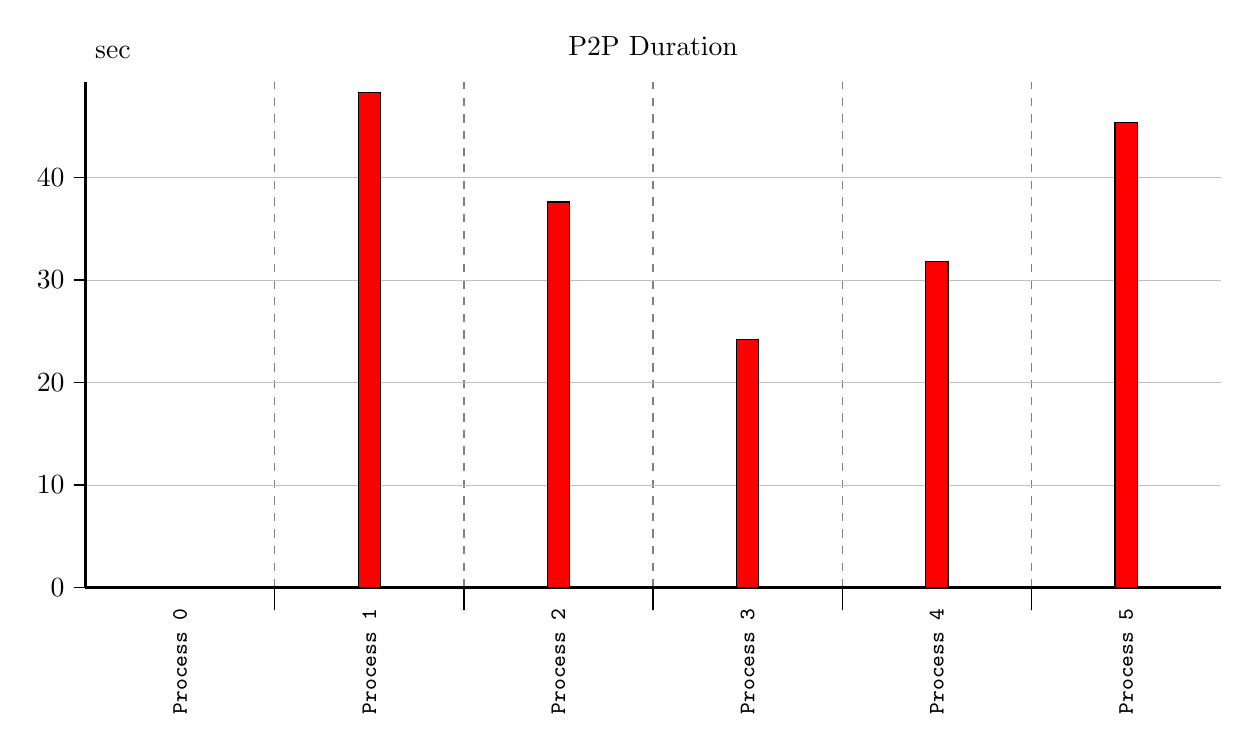
\begin{tikzpicture}
\begin{axis}[
  width=16cm, height=8cm,
  axis x line=bottom,x axis line style={-,line width=1pt},
  axis y line=left,y axis line style={-,line width=1pt},
  enlarge y limits={value=0.02,upper},
ymin=0,
  ylabel style={at={(0,7cm)},rotate=-90,anchor=north west},
ymajorgrids,xminorgrids,minor x tick num=1,
title=P2P Duration,ylabel={sec},
x tick label style={rotate=90,anchor=east,font=\ttfamily\footnotesize},
tick align=outside,
tick style={line cap=round,line width=0.5pt,color=black,
      major tick length=4pt,minor tick length=8pt},
major x tick style={line width=1, color=white},
scaled y ticks=true,
bar width=8pt,
minor grid style={color=gray, line width=0.5pt, dashed},
xmin=-0.5,
xmax=5.5,
xtick={0,...,5},
xticklabels={
Process 0,Process 1,Process 2,Process 3,Process 4,Process 5,},]
\addplot[ybar, draw=black, mark=none, fill=red]
  coordinates{
(1,48.3365712)(2,37.6133575)(3,24.1584843)(4,31.7870589)(5,45.3695342)};
\end{axis}
\end{tikzpicture}

\end{flushright}
\begin{flushright}
\bigskip

\begin{tikzpicture}
\node(a) at (0,0) [rectangle, draw, fill=red] {};
\node [black,right] at (a.east) {send};
\node(b) at (2,0) [rectangle, draw, fill=blue] {};
\node [black,right] at (b.east) {receive};
\end{tikzpicture}
\end{flushright}
\newpage

\center{\Large \bf P2P - Message Rate Histogram}
\bigskip

\begin{center}
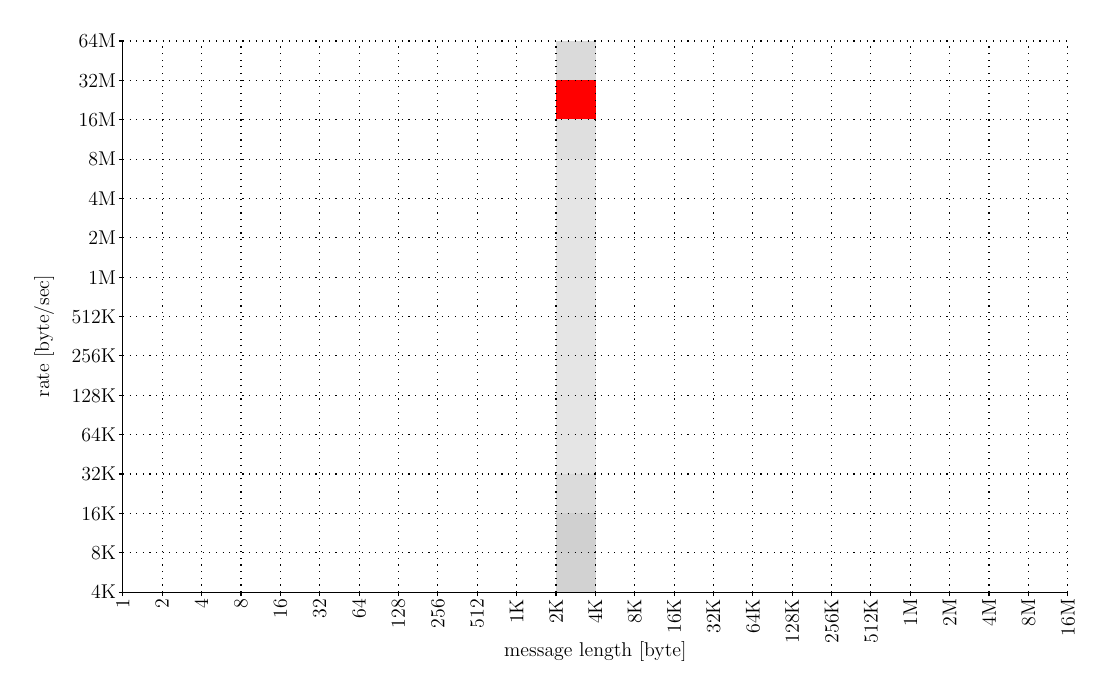
\begin{tikzpicture} [step=1cm,scale=0.5,every node/.style={scale=0.5}]\Large
\node[minimum size=1cm,anchor=south west] at (11,0) [rectangle, fill={rgb,1:red,0.825504;green,0.825504;blue,0.825504}] {};
\node[minimum size=1cm,anchor=south west] at (11,1) [rectangle, fill={rgb,1:red,0.813962;green,0.813962;blue,0.813962}] {};
\node[minimum size=1cm,anchor=south west] at (11,2) [rectangle, fill={rgb,1:red,0.859779;green,0.859779;blue,0.859779}] {};
\node[minimum size=1cm,anchor=south west] at (11,3) [rectangle, fill={rgb,1:red,0.896502;green,0.896502;blue,0.896502}] {};
\node[minimum size=1cm,anchor=south west] at (11,4) [rectangle, fill={rgb,1:red,0.898251;green,0.898251;blue,0.898251}] {};
\node[minimum size=1cm,anchor=south west] at (11,5) [rectangle, fill={rgb,1:red,0.899301;green,0.899301;blue,0.899301}] {};
\node[minimum size=1cm,anchor=south west] at (11,6) [rectangle, fill={rgb,1:red,0.897902;green,0.897902;blue,0.897902}] {};
\node[minimum size=1cm,anchor=south west] at (11,7) [rectangle, fill={rgb,1:red,0.896852;green,0.896852;blue,0.896852}] {};
\node[minimum size=1cm,anchor=south west] at (11,8) [rectangle, fill={rgb,1:red,0.894754;green,0.894754;blue,0.894754}] {};
\node[minimum size=1cm,anchor=south west] at (11,9) [rectangle, fill={rgb,1:red,0.897552;green,0.897552;blue,0.897552}] {};
\node[minimum size=1cm,anchor=south west] at (11,10) [rectangle, fill={rgb,1:red,0.897552;green,0.897552;blue,0.897552}] {};
\node[minimum size=1cm,anchor=south west] at (11,11) [rectangle, fill={rgb,1:red,0.873069;green,0.873069;blue,0.873069}] {};
\node[minimum size=1cm,anchor=south west] at (11,12) [rectangle, fill={rgb,1:red,1.000000;green,0.000000;blue,0.000000}] {};
\node[minimum size=1cm,anchor=south west] at (11,13) [rectangle, fill={rgb,1:red,0.855932;green,0.855932;blue,0.855932}] {};
\draw (0,-0.1) -- (0,0) node[rotate=90,left] at (0,0) {1};
\draw (1,-0.1) -- (1,0) node[rotate=90,left] at (1,0) {2};
\draw (2,-0.1) -- (2,0) node[rotate=90,left] at (2,0) {4};
\draw (3,-0.1) -- (3,0) node[rotate=90,left] at (3,0) {8};
\draw (4,-0.1) -- (4,0) node[rotate=90,left] at (4,0) {16};
\draw (5,-0.1) -- (5,0) node[rotate=90,left] at (5,0) {32};
\draw (6,-0.1) -- (6,0) node[rotate=90,left] at (6,0) {64};
\draw (7,-0.1) -- (7,0) node[rotate=90,left] at (7,0) {128};
\draw (8,-0.1) -- (8,0) node[rotate=90,left] at (8,0) {256};
\draw (9,-0.1) -- (9,0) node[rotate=90,left] at (9,0) {512};
\draw (10,-0.1) -- (10,0) node[rotate=90,left] at (10,0) {1K};
\draw (11,-0.1) -- (11,0) node[rotate=90,left] at (11,0) {2K};
\draw (12,-0.1) -- (12,0) node[rotate=90,left] at (12,0) {4K};
\draw (13,-0.1) -- (13,0) node[rotate=90,left] at (13,0) {8K};
\draw (14,-0.1) -- (14,0) node[rotate=90,left] at (14,0) {16K};
\draw (15,-0.1) -- (15,0) node[rotate=90,left] at (15,0) {32K};
\draw (16,-0.1) -- (16,0) node[rotate=90,left] at (16,0) {64K};
\draw (17,-0.1) -- (17,0) node[rotate=90,left] at (17,0) {128K};
\draw (18,-0.1) -- (18,0) node[rotate=90,left] at (18,0) {256K};
\draw (19,-0.1) -- (19,0) node[rotate=90,left] at (19,0) {512K};
\draw (20,-0.1) -- (20,0) node[rotate=90,left] at (20,0) {1M};
\draw (21,-0.1) -- (21,0) node[rotate=90,left] at (21,0) {2M};
\draw (22,-0.1) -- (22,0) node[rotate=90,left] at (22,0) {4M};
\draw (23,-0.1) -- (23,0) node[rotate=90,left] at (23,0) {8M};
\draw (24,-0.1) -- (24,0) node[rotate=90,left] at (24,0) {16M};
\draw (-0.1,0) -- (0,0) node[anchor=east] at (0,0) {4K};
\draw (-0.1,1) -- (0,1) node[anchor=east] at (0,1) {8K};
\draw (-0.1,2) -- (0,2) node[anchor=east] at (0,2) {16K};
\draw (-0.1,3) -- (0,3) node[anchor=east] at (0,3) {32K};
\draw (-0.1,4) -- (0,4) node[anchor=east] at (0,4) {64K};
\draw (-0.1,5) -- (0,5) node[anchor=east] at (0,5) {128K};
\draw (-0.1,6) -- (0,6) node[anchor=east] at (0,6) {256K};
\draw (-0.1,7) -- (0,7) node[anchor=east] at (0,7) {512K};
\draw (-0.1,8) -- (0,8) node[anchor=east] at (0,8) {1M};
\draw (-0.1,9) -- (0,9) node[anchor=east] at (0,9) {2M};
\draw (-0.1,10) -- (0,10) node[anchor=east] at (0,10) {4M};
\draw (-0.1,11) -- (0,11) node[anchor=east] at (0,11) {8M};
\draw (-0.1,12) -- (0,12) node[anchor=east] at (0,12) {16M};
\draw (-0.1,13) -- (0,13) node[anchor=east] at (0,13) {32M};
\draw (-0.1,14) -- (0,14) node[anchor=east] at (0,14) {64M};
\draw (-0.1,0) -- (24,0);
\draw (0,-0.1) -- (0,14); %y axis
\draw[dotted] (0,0) grid (24,14);
\node[rotate=90] at (-2,6.5) {rate [byte/sec]};
\node at (12, -1.5) {message length [byte]};
\end{tikzpicture}\bigskip

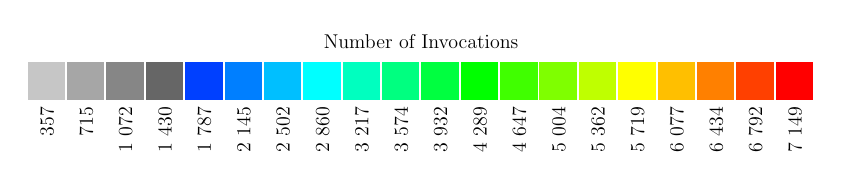
\begin{tikzpicture} [step=1cm,scale=0.5,every node/.style={scale=0.5}]\Large
\node at (11, 0) {Number of Invocations};
\node[minimum size=0.95cm,anchor=south west] at (1,-1.5) [rectangle, fill={rgb,1:red,0.775332 ;green,0.775332;blue,0.775332}] {};
\node[anchor=east,rotate=90] at (1.500000,-1.5) {357};
\node[minimum size=0.95cm,anchor=south west] at (2,-1.5) [rectangle, fill={rgb,1:red,0.650315 ;green,0.650315;blue,0.650315}] {};
\node[anchor=east,rotate=90] at (2.500000,-1.5) {715};
\node[minimum size=0.95cm,anchor=south west] at (3,-1.5) [rectangle, fill={rgb,1:red,0.525297 ;green,0.525297;blue,0.525297}] {};
\node[anchor=east,rotate=90] at (3.500000,-1.5) {1 072};
\node[minimum size=0.95cm,anchor=south west] at (4,-1.5) [rectangle, fill={rgb,1:red,0.400280 ;green,0.400280;blue,0.400280}] {};
\node[anchor=east,rotate=90] at (4.500000,-1.5) {1 430};
\node[minimum size=0.95cm,anchor=south west] at (5,-1.5) [rectangle, fill={rgb,1:red,0.000000 ;green,0.249475;blue,1.000000}] {};
\node[anchor=east,rotate=90] at (5.500000,-1.5) {1 787};
\node[minimum size=0.95cm,anchor=south west] at (6,-1.5) [rectangle, fill={rgb,1:red,0.000000 ;green,0.499510;blue,1.000000}] {};
\node[anchor=east,rotate=90] at (6.500000,-1.5) {2 145};
\node[minimum size=0.95cm,anchor=south west] at (7,-1.5) [rectangle, fill={rgb,1:red,0.000000 ;green,0.749545;blue,1.000000}] {};
\node[anchor=east,rotate=90] at (7.500000,-1.5) {2 502};
\node[minimum size=0.95cm,anchor=south west] at (8,-1.5) [rectangle, fill={rgb,1:red,0.000000 ;green,0.999580;blue,1.000000}] {};
\node[anchor=east,rotate=90] at (8.500000,-1.5) {2 860};
\node[minimum size=0.95cm,anchor=south west] at (9,-1.5) [rectangle, fill={rgb,1:red,0.000000 ;green,1.000000;blue,0.750385}] {};
\node[anchor=east,rotate=90] at (9.500000,-1.5) {3 217};
\node[minimum size=0.95cm,anchor=south west] at (10,-1.5) [rectangle, fill={rgb,1:red,0.000000 ;green,1.000000;blue,0.500350}] {};
\node[anchor=east,rotate=90] at (10.500000,-1.5) {3 574};
\node[minimum size=0.95cm,anchor=south west] at (11,-1.5) [rectangle, fill={rgb,1:red,0.000000 ;green,1.000000;blue,0.250315}] {};
\node[anchor=east,rotate=90] at (11.500000,-1.5) {3 932};
\node[minimum size=0.95cm,anchor=south west] at (12,-1.5) [rectangle, fill={rgb,1:red,0.000000 ;green,1.000000;blue,0.000280}] {};
\node[anchor=east,rotate=90] at (12.500000,-1.5) {4 289};
\node[minimum size=0.95cm,anchor=south west] at (13,-1.5) [rectangle, fill={rgb,1:red,0.249755 ;green,1.000000;blue,0.000000}] {};
\node[anchor=east,rotate=90] at (13.500000,-1.5) {4 647};
\node[minimum size=0.95cm,anchor=south west] at (14,-1.5) [rectangle, fill={rgb,1:red,0.499790 ;green,1.000000;blue,0.000000}] {};
\node[anchor=east,rotate=90] at (14.500000,-1.5) {5 004};
\node[minimum size=0.95cm,anchor=south west] at (15,-1.5) [rectangle, fill={rgb,1:red,0.749825 ;green,1.000000;blue,0.000000}] {};
\node[anchor=east,rotate=90] at (15.500000,-1.5) {5 362};
\node[minimum size=0.95cm,anchor=south west] at (16,-1.5) [rectangle, fill={rgb,1:red,0.999860 ;green,1.000000;blue,0.000000}] {};
\node[anchor=east,rotate=90] at (16.500000,-1.5) {5 719};
\node[minimum size=0.95cm,anchor=south west] at (17,-1.5) [rectangle, fill={rgb,1:red,1.000000 ;green,0.750105;blue,0.000000}] {};
\node[anchor=east,rotate=90] at (17.500000,-1.5) {6 077};
\node[minimum size=0.95cm,anchor=south west] at (18,-1.5) [rectangle, fill={rgb,1:red,1.000000 ;green,0.500070;blue,0.000000}] {};
\node[anchor=east,rotate=90] at (18.500000,-1.5) {6 434};
\node[minimum size=0.95cm,anchor=south west] at (19,-1.5) [rectangle, fill={rgb,1:red,1.000000 ;green,0.250035;blue,0.000000}] {};
\node[anchor=east,rotate=90] at (19.500000,-1.5) {6 792};
\node[minimum size=0.95cm,anchor=south west] at (20,-1.5) [rectangle, fill={rgb,1:red,1.000000 ;green,0.000000;blue,0.000000}] {};
\node[anchor=east,rotate=90] at (20.500000,-1.5) {7 149};
\end{tikzpicture}
\end{center}
\newpage
\pgfplotstableread{
group cntSend cntRecv bytSend bytRecv durSend durRecv
0 10 10 0 0 0.00213843294 0.00213843294
1 10 10 0 0 5.0043732 5.0043732
2 10 10 0 0 3.35683776 3.35683776
3 10 10 0 0 0.518557057 0.518557057
4 10 10 0 0 1.07329388 1.07329388
5 10 10 0 0 2.48091044 2.48091044
}\BARRIER
\begin{flushright}\ttfamily\small
\begin{tikzpicture}
\begin{axis}[
  width=16cm, height=8cm,
  axis x line=bottom,x axis line style={-,line width=1pt},
  axis y line=left,y axis line style={-,line width=1pt},
  enlarge y limits={value=0.02,upper},
  ymin=0,ymajorgrids,xminorgrids,minor x tick num=1,
title=BARRIER Invocations,ylabel={},
x tick label style={rotate=90,anchor=east,font=\ttfamily\footnotesize},
tick align=outside,
tick style={line cap=round,line width=0.5pt,color=black,
      major tick length=4pt,minor tick length=8pt},
major x tick style={line width=1, color=white},
scaled y ticks=true,
bar width=8pt,
minor grid style={color=gray, line width=0.5pt, dashed},
xmin=-0.5,
xmax=5.5,
xtick={0,...,5},
xticklabels={
},]
\addplot[ybar, draw=black, mark=none, fill=red] table[x=group,y=cntSend] {\BARRIER};
\end{axis}
\end{tikzpicture}

\end{flushright}
\begin{flushright}\ttfamily\small
\begin{tikzpicture}
\begin{axis}[
  width=16cm, height=8cm,
  axis x line=bottom,x axis line style={-,line width=1pt},
  axis y line=left,y axis line style={-,line width=1pt},
  enlarge y limits={value=0.02,upper},
ymin=0,
  ylabel style={at={(0,7cm)},rotate=-90,anchor=north west},
ymajorgrids,xminorgrids,minor x tick num=1,
title=BARRIER Duration,ylabel={sec},
x tick label style={rotate=90,anchor=east,font=\ttfamily\footnotesize},
tick align=outside,
tick style={line cap=round,line width=0.5pt,color=black,
      major tick length=4pt,minor tick length=8pt},
major x tick style={line width=1, color=white},
scaled y ticks=true,
bar width=8pt,
minor grid style={color=gray, line width=0.5pt, dashed},
xmin=-0.5,
xmax=5.5,
xtick={0,...,5},
xticklabels={
Process 0,Process 1,Process 2,Process 3,Process 4,Process 5,},]
\addplot[ybar, draw=black, mark=none, fill=red] table[x=group,y=durSend] {\BARRIER};
\end{axis}
\end{tikzpicture}

\end{flushright}
\begin{flushright}
\bigskip
\begin{tikzpicture}
\end{tikzpicture}
\end{flushright}
\newpage


\end{document}
